\chapter{The Broadcast}
\label{ch:25}



\begin{center}
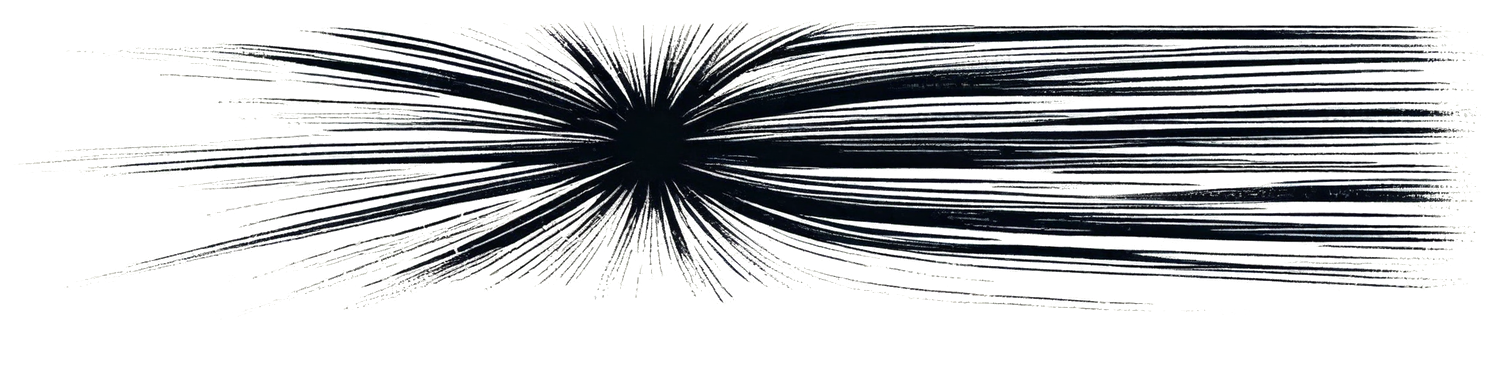
\includegraphics[width=\textwidth]{images/chapterImages/genesis_sketch_00122_.png}
\end{center}

The video was simple. No special effects. No dramatic music. Just Sarah Chen sitting in a plain room with a camera and the weight of 65 million years of genetic programming on her shoulders.

She'd recorded it seventeen times. Each version different. Each attempt trying to find the right tone. The right words. The right way to tell humanity that everything they thought about themselves was wrong.

This was take eighteen. The final version. The one they'd decided to release.

Sarah looked at the camera. Took a breath. Began.

"My name is Dr. Sarah Chen. I'm a geneticist. For the past three years, I've been studying patterns in human DNA that don't make sense according to conventional evolutionary theory. Today I'm going to tell you what I found. And I need you to understand: this is not speculation. This is not theory. This is verified, peer-reviewed fact supported by evidence from multiple independent research teams across the globe."

She paused. Let that settle. Let people understand this was serious.

"65 million years ago, an intelligent species existed on Earth. Not humans. Not mammals. A species of reptilian intelligence that we've come to call 'The Architects.' They were brilliant. Capable of complex calculation, long-term planning, and—critically—genetic engineering at a level we're only beginning to understand."

Another pause. She could feel the weight of what came next. The revelation that would break everything.

"The Architects detected an incoming asteroid. They calculated impact probability at near 100\%. They knew they were going to die. They couldn't save themselves. But they could save the planet. They could encode planetary defense capability into small mammals that would survive the extinction event. They could program evolution. Program capability. Program *us*."

Sarah pulled up images. DNA sequences. Activation markers. Mathematical proofs.

"This is what they did. They modified mammalian DNA to include specific capability thresholds. Tool use. Fire. Agriculture. Writing. Mathematics. Astronomy. And finally—planetary defense. Each capability encoded to activate when environmental conditions triggered it. Each threshold timed to ensure maximum survival probability."

She let the images show. Let people see the evidence. The mathematical precision. The undeniable patterns.

"Human evolution is not random. It's programmed. Every major capability—from using rocks as tools to building space telescopes—was encoded into our DNA 65 million years ago by beings who died to ensure we could do what they couldn't: protect this planet from extinction."

Now came the hard part. The personal cost. The compulsion.

"Three years ago, I discovered this. Two years ago, I began experiencing what we call 'activation.' A neurological compulsion to work on planetary defense systems. Not a suggestion. Not inspiration. A drive so powerful I cannot resist it. I stopped sleeping normally. Stopped eating regularly. Stopped being present for my daughter. Not because I chose to—though choice is complicated—but because the activation made everything except the work feel irrelevant."

Sarah felt her voice crack. Stopped. Composed herself.

"I'm not alone. Thousands of people globally have experienced the same activation. Engineers. Physicists. Mathematicians. All driven to work on the same project. All unable to stop. All sacrificing relationships, careers, health. We're building a planetary defense grid. And we can't choose not to."

She pulled up statistics. Relationship endings. Job losses. Hospitalizations. The cost visible in data.

"The activation has destroyed lives. Ended marriages. Traumatized children. People have died—from exhaustion, from accidents while compulsively working, from suicide after trying to resist. This is the cost of using the capability The Architects gave us."

Sarah looked directly at the camera. Made eye contact with the millions who would watch this.

"I'm telling you this because you deserve to know. Because humanity deserves the truth. And because there's an asteroid coming. 2027 RL₃. Impact probability 94.3\%. Time to impact: 38 years, 7 months. The planetary defense grid we're building—the one we're compelled to build—might be humanity's only chance at survival."

She pulled up the asteroid data. Trajectory calculations. Impact projections.

"The Architects knew. They calculated this. They encoded the capability to activate exactly when we'd need it. The program is executing perfectly. We're doing exactly what we were designed to do. And it's working."

Sarah paused again. This next part was critical.

"Now you're going to ask: do we have free will? If our capabilities are programmed, are our choices real? I've spent three years trying to answer that question. The honest answer is: I don't know. The capability is programmed. The compulsion is real. But the person experiencing the compulsion is also real. The suffering is real. The love I feel for my daughter—even though I can't be present for her—is real. Whether that means free will exists or just that the programming is sophisticated enough to create the illusion of choice... I don't know."

She felt tears coming. Didn't stop them. Let them show.

"What I do know is this: The Architects loved this planet enough to die for it. Loved it enough to spend their final years programming our future instead of enjoying their remaining time. They gave us a gift. A terrible, beautiful, devastating gift. The capability to survive when they couldn't. And I believe—I choose to believe—that using that gift honors what they did for us."

Sarah composed herself. Final section.

"Over the next few weeks, months, years, you're going to learn more. Research papers will be published. Evidence will be analyzed. Debates will happen. Some people will deny this. Some will embrace it. Some will spiral into despair. All of those responses are valid. This is hard information. It changes everything."

She looked at the camera. Tried to project something like compassion. Like understanding.

"But humanity is still here. Still conscious. Still capable of asking whether any of this matters. And I think—I hope—that the capacity to question our own programming might be the thing that makes us real. That makes us more than just code executing."

Final breath. Final statement.

"The defense grid is being built. The asteroid will be deflected. Humanity will survive. And we'll survive knowing what we are. Programmed. Capable. Conscious. All of it simultaneously. All of it real. That's what The Architects gave us. That's what we're choosing to use. And whatever happens next—whatever philosophy emerges, whatever meaning we construct—will be ours to determine. As much as anything can be ours."

Sarah stopped. Turned off the camera. Sat in silence.

It was done. The truth told. The revelation made.

No taking it back. No controlling the response. No knowing what would happen next.

\scenebreak

The video released simultaneously across every major platform. News networks. Social media. Academic channels. Government feeds. Coordinated global release. Maximum impact. No way to suppress it.

Within an hour: 50 million views.

Within two hours: 200 million.

Within six hours: trending on every platform. The top story globally. The only story that mattered.

The response was immediate and chaotic.

Denial came first. This had to be hoax. Had to be misinformation. Genetic patterns couldn't be that precise. Evolution didn't work that way. Someone was lying.

But the evidence was public. The DNA sequences available. The mathematical proofs verifiable. Dozens of independent research teams confirming the findings.

The denial couldn't hold. The evidence was too strong. The patterns too obvious once you knew to look for them.

After denial: anger.

Rage at the researchers for revealing it. Rage at The Architects for programming humanity. Rage at universities for hiding this. Rage at governments for not disclosing sooner. Rage at activated individuals for being compelled. Rage at God for allowing this. Rage at existence for being programmable.

The anger expressed in protests. In violence. In targeted harassment of researchers. Sarah's home address leaked within hours. Marcus's warehouse vandalized. Katherine receiving death threats.

People screaming that free will was sacred. That this revelation stole meaning. That humans were supposed to be special. That being programmed made them slaves.

After anger: grief.

Mass grieving for the loss of human specialness. For the illusion of autonomy. For the belief that achievements were chosen. For the comfort of thinking consciousness was free.

Suicide rates spiked. Hospitals overflowed with people experiencing existential crises. Therapists overwhelmed. Crisis hotlines jammed. The psychological cost of knowing becoming immediately visible.

Children asking parents if their love was real. Couples questioning whether relationships were choice or programming. Artists wondering if creativity was authentic or just activation. Scientists doubting whether discoveries were genius or genetic expression.

Everything called into question. Every assumption challenged. Every certainty dissolved.

And through it all: the activated kept working. The compulsion didn't stop for revelation. Didn't pause for global crisis. The grid continued being built. The work continued.

\scenebreak

Sarah's apartment was no longer safe. She'd moved to secure facility. Armed guards. Controlled access. Twenty-four-hour protection.

She watched the global response on screens. Saw the rage. Saw the grief. Saw humanity fracturing under the weight of truth.

Her phone—switched to a new number, known only to family—rang.

Tom.

"Sarah. I just... I saw the video. Saw the evidence. Is this real? Is all of this actually real?"

"Yes."

"And you've known for three years?"

"Yes."

"And you couldn't tell us. Couldn't tell Maya. Couldn't warn anyone this was coming?"

"We were trying to find the right way. Trying to minimize harm. Trying to—"

"There's no right way to tell people they're programmed, Sarah! There's no good version of this revelation!"

She heard the pain in his voice. The betrayal. The anger.

"I know."

"Maya is devastated. Asking if she's real. Asking if I love her because I want to or because I'm programmed to. Asking if anything means anything. She's eight years old and you've destroyed her sense of reality."

"Tom, I'm sorry. I'm so sorry. But the asteroid is real. The threat is real. Humanity needs to build the defense. Needs to understand why some people can't stop working. This revelation was necessary."

"Necessary for who? For you? For your work? How is any of this more important than my daughter's mental health?"

"Our daughter. She's our daughter, Tom."

"You lost the right to claim her when you chose the work. When you let the compulsion win. When you decided saving humanity was more important than being her mother."

Sarah felt something break. Different than before. Worse than before. The finality of it.

"Tom, please—"

"I'm done, Sarah. Maya is done. Don't call us. Don't try to explain. Don't send messages about programming and compulsion and genetic inheritance. We're moving on. Living our lives. Trying to find meaning in a world that apparently has none."

He hung up. Sarah sat in silence. Staring at her phone. Knowing she'd lost her daughter. Lost her permanently. No going back. No repair possible.

The cost of disclosure measured in one eight-year-old girl who no longer believed love was real.

\scenebreak

The philosophical community erupted. Decades of debate about free will suddenly made obsolete. The determinists were right. Sort of. The compatibilists scrambling to adapt. The libertarian free will advocates devastated.

Papers published overnight. Conferences called. Universities offering crisis counseling for philosophy students whose entire field had just been redefined.

Religious responses varied wildly. Some denominations claiming this proved God—that God had used The Architects as instruments. Others declaring it disproved God—that genetic programming explained everything. Others still insisting human souls transcended programming—that consciousness was more than code.

The Vatican issued a statement: "The revelation of genetic programming does not diminish the spiritual nature of humanity. We are still God's children, even if the mechanism of our creation is more complex than previously understood."

Not everyone found that comforting.

Mosques. Temples. Synagogues. All grappling with the revelation. All trying to preserve meaning while acknowledging programming. All losing congregants who couldn't reconcile faith with genetic determinism.

Atheist communities had their own crisis. Many had argued for free will despite lack of souls. Now forced to confront evidence that choice might be illusion. That consciousness might be sophisticated programming. That meaning might be subjective construction with no objective basis.

Everyone struggling. Everyone questioning. Everyone trying to find ground under feet that had been pulled away.

\scenebreak

Governments responded with predictable chaos. Some demanding the defense grid stop. Some demanding it accelerate. Some trying to take control. Some denying the asteroid was real.

The UN called emergency session. 193 member states trying to determine collective response. Trying to decide whether to support activated individuals or restrict them. Trying to figure out if programming was slavery or duty.

No consensus emerged. Just fracture. Division. Each nation responding according to its own values, its own fears, its own interpretation of what this revelation meant.

China announced full state support for activated individuals. Mandatory protection. Mandatory resources. Treating the compulsion as national service. Conscripting the activated into defense grid construction.

The US couldn't decide. Federal government paralyzed by debate. States implementing their own policies. Some protecting activated individuals. Some criminalizing the work. Some trying to study them. Some trying to eliminate them.

Europe split. Some nations embracing the revelation. Some rejecting it. Some trying to find middle ground between acceptance and denial.

Global coordination—the thing the defense grid desperately needed—dissolved into chaos. Each nation choosing its own path. Each response different. Each interpretation unique.

The asteroid kept coming. 38 years, 7 months. Then 38 years, 6 months. Then 38 years, 5 months.

Time passing. Crisis continuing. Humanity fracturing while the clock ran down.

\scenebreak

Marcus watched the response from his warehouse. Saw the riots on news feeds. Saw the rage directed at activated individuals. Saw people calling them traitors for revealing the truth.

His warehouse had been vandalized twice. Death threats arriving daily. Other activated individuals reporting similar harassment. Some murdered by people who thought killing the compelled would somehow restore free will.

It was irrational. It was understandable. It was human.

Marcus thought about David. Wondered if David had seen the broadcast. Wondered if he understood now. Wondered if understanding changed anything.

He pulled up David's contact. Stared at it. Thought about calling. Couldn't do it. The compulsion pulling him back to work. Always back to work.

Instead he sent a text: *I saw your message. From the celebration announcement. I understand now why you said that. I'm sorry I couldn't choose you. Sorry I couldn't be what you needed. The broadcast explains why. Doesn't excuse it. Just explains it. I think about you every day. Hope you're okay.*

He hit send. Returned to work. The compulsion immediate. Overwhelming. Necessary.

His phone buzzed. David responding: *I saw the broadcast. I understand. Doesn't make it hurt less. But I understand. I'm alive. I'm okay. I hope you're safe. I hope you finish the grid. I hope it works. And I hope afterward—if there is an afterward—you find whatever peace programmed beings can find.*

Marcus read it three times. Felt something. Couldn't name it. Returned to work.

The response was what it was. The cost was what it was. The compulsion continued. The work continued. The grid advanced.

And 38 years, 7 months became 38 years, 6 months, 29 days. The asteroid approaching. The clock running. The world fracturing while humanity tried to survive knowing what it was.

\scenebreak

Three months after the broadcast, the global response had stabilized into three camps:

Acceptance: Those who embraced the revelation. Who found meaning in being programmed. Who chose to honor The Architects' gift. Who worked to support activated individuals and build the defense grid.

Roughly 35\% of humanity.

Denial: Those who refused to believe. Who insisted the evidence was fabricated. Who clung to free will despite proof. Who rejected the programming explanation.

Roughly 40\% of humanity.

Resistance: Those who acknowledged the programming but fought against it. Who insisted humans should reject genetic compulsion. Who tried to stop the defense grid. Who chose death over being tools.

Roughly 25\% of humanity.

The camps didn't align with national borders. Didn't align with religious traditions. Didn't align with political ideologies. Each individual responding according to something deeper. Something personal. Something that might have been choice or might have been programming.

No one knew. No one could know. That was the horror and the beauty of it.

Sarah watched the camps form. Watched humanity divide. Watched her revelation create exactly the crisis Katherine had warned about.

She regretted nothing. Regretted everything. Regretted that regret was ambiguous.

The truth was told. The cost paid. The response happening. Humanity choosing—or failing to choose—how to proceed.

And the activated kept working. The grid kept advancing. The capability kept expressing.

Because 38 years wasn't long. Because the asteroid was real. Because The Architects had programmed this exact response for this exact moment.

Because the compulsion didn't care about chaos. Didn't care about philosophical crisis. Didn't care about anything except completion.

The broadcast had happened. The truth was known. The fracture was real.

And humanity moved forward into unknown territory. Aware. Programmed. Suffering. Surviving.

All of it simultaneously. All of it necessary. All of it chosen by beings who couldn't know if choice was real but chose anyway.

The program executed. The response unfolded. The work continued.

And Sarah Chen, having told the truth that destroyed everything, returned to the compulsion that defined her.

Because the asteroid was coming. Because the grid needed building. Because 38 years, 6 months, 29 days was shorter than 38 years, 7 months.

Because the work was all she had. All anyone had. All that mattered.

The mathematics was complete. The truth was told. The cost was paid.

And humanity built its defense while arguing about whether building it was choice.

The program continued. The clock ran. The future approached.

One day at a time. One calculation at a time. One completed component at a time.

Until the grid was done. Until the asteroid was deflected. Until The Architects' program completed.

Or until humanity destroyed itself trying to prove it wasn't programmed.

Whichever came first.

The broadcast was complete. The revelation made. The response unfolding.

And Sarah Chen, mother and scientist and tool, worked through the chaos she'd created.

Because she had to. Because she chose to. Because the distinction no longer mattered.

The truth was told. The world was changed. The work continued.

Forever. Until completion. Whichever came first.

